\documentclass{article}

\usepackage{amsmath,amssymb}
\usepackage{tikz}
\usepackage{pgfplots}
\usepackage{xcolor}
\usepackage[left=2.1cm,right=3.1cm,bottom=3cm,footskip=0.75cm,headsep=0.5cm]{geometry}
\usepackage{enumerate}
\usepackage{enumitem}
\usepackage{marvosym}
\usepackage{tabularx}
\usepackage{multirow}
\usepackage[colorlinks = true, linkcolor = blue, urlcolor  = blue, citecolor = blue, anchorcolor = blue]{hyperref}
\usepackage{ulem}

\usepackage{listings}
\definecolor{lightlightgray}{rgb}{0.95,0.95,0.95}
\definecolor{lila}{rgb}{0.8,0,0.8}
\definecolor{mygray}{rgb}{0.5,0.5,0.5}
\definecolor{mygreen}{rgb}{0,0.8,0.26}
\lstdefinestyle{java} {language=java}
\lstset{language=java,
	basicstyle=\ttfamily,
	keywordstyle=\color{lila},
	commentstyle=\color{lightgray},
	stringstyle=\color{mygreen}\ttfamily,
	backgroundcolor=\color{white},
	showstringspaces=false,
	numbers=left,
	numbersep=10pt,
	numberstyle=\color{mygray}\ttfamily,
	identifierstyle=\color{blue},
	xleftmargin=.1\textwidth, 
	%xrightmargin=.1\textwidth,
	escapechar=§,
}

\usepackage[utf8]{inputenc}

\renewcommand*{\arraystretch}{1.4}

\newcolumntype{L}[1]{>{\raggedright\arraybackslash}p{#1}}
\newcolumntype{R}[1]{>{\raggedleft\arraybackslash}p{#1}}
\newcolumntype{C}[1]{>{\centering\let\newline\\\arraybackslash\hspace{0pt}}m{#1}}

\newcommand{\E}{\mathbb{E}}
\DeclareMathOperator{\rk}{rk}
\DeclareMathOperator{\Var}{Var}
\DeclareMathOperator{\Cov}{Cov}
\DeclareMathOperator{\SD}{SD}
\DeclareMathOperator{\Cor}{Cor}

\title{\textbf{Mensch-Computer-Interaktion, Übung 1}}
\author{\textsc{Henry Haustein}, \textsc{Dennis Rössel}}
\date{}

\begin{document}
	\maketitle
	
	\section*{Aufgabe 1.1: Sammlung von Methoden recherchieren}
	\begin{enumerate}[label=(\alph*)]
		\item Kontextanalyse: Aus Informationen über die zukünftigen Benutzer soll ein Verständnis des Use-Cases der Anwendung ermittelt entstehen. Dazu können Interviews oder Umfragen genutzt werden. Einsatz in der frühen Phase des Projektes.
		\item Benutzendenanalyse: Ziel sind mögliche Designideen und Lösungen die im preislichen Rahmen liegen. Dazu muss erfasst werden, welche Präferenzen die Nutzer haben, also was ihnen wichtig ist. Auch das findet in der frühen Phase des Projektes statt und kann durch Fokusgruppen und Interviews erledigt werden.
		\item Designmethoden: In dieser Phase wird die Designidee aus der vorherigen Phase in einer Entwicklungsumgebung umgesetzt. Hierfür gibt es verschiedene Methoden, z.B. Prototyping oder auch das V-Modell. Das findet in der Hauptphase des Projektes statt.
		\item Evaluation: Die Software wird an den tatsächlichen späteren Nutzern getestet und deren Feedback wird verwendet um die Software in der nächsten Iteration zu verbessern. Usebility-Test, zum Beispiel unter anderem mit Eye-Tracking.
	\end{enumerate}
	Die ersten beiden Phasen können auch 50\% des zeitlichen und preislichen Aufwandes eines Projektes ausmachen!

	\section*{Aufgabe 1.2: Einbettung des UCD-Prozesses in ein Softwareprojekt}
	\begin{enumerate}[label=(\alph*)]
		\item Prinzipiell kann in Entwicklung jeder Software, mit der ein User interagieren kann, ein UCD-Prozess eingebunden werden (und sollte auch!).
		\item Für reine Backend-Lösungen kann kein UCD-Prozess durchgeführt werden, da z.B. die Evaluation durch Nutzer komplett wegfällt.
		\item Integration von UCD in klassische Entwicklungsprozesse, am Beispiel des Wasserfallmodells: Es müssen Iterationen ins Wasserfallmodell eingebaut werden, insbesondere müsste vor der Inbetriebnahme noch eine Evaluation durchgeführt werden und Fehler müssen beseitigt werden. Dazu kann es nötig sein, nochmals in eine viel frühere Phase des Wasserfallsmodells zurückzugehen. Zudem muss der Fokus des Wasserfallmodells weg von der Dokumentation hin zur Interaktion mit dem zukünftigen User gelegt werden.
		\item Integration von UCD in agile Entwicklungsprozesse, am Beispiel von Scrum: Scrum bietet einen sehr guten iterativen Entwicklungsprozess, aber es fehlen Kontextanalyse und Benutzendenanalyse. Nach jedem Sprint erfolgt eine Evaluation mit anschließendem Zurückkehren zur Kontextanalyse/Benutzendenanalyse.
	\end{enumerate}
	
	\section*{Aufgabe 1.3: Projektidee}
	\begin{enumerate}[label=(\alph*)]
		\item unsere 5 Ideen:
		\begin{itemize}
			\item Telefonclient, um mit der Büronummer auch unterwegs erreichbar zu sein. Platform: Software für die Telefonanlage und eine Handyapp, Zielgruppe: Berufstätige
			\item Webapp, damit sich von der Unternehmenswebseite direkt Supporttickets erstellen lassen. Platform: Webapp, Zielgruppe: Unternehmen mit Ticketsystem und unzufriedenen Kunden
			\item \textbf{soziales Netzwerk exklusiv für Studierende. Platform: Webseite + Handyapp, Zielgruppe: Studenten}
			\item Webapp, mit der sich die meisten Aufgaben aus Altklausuren schnell und effizient \sout{während der Klausur} als Klausurvorbereitung lösen lassen inklusive Lösungsweg. Platform: Webapp, Zielgruppe: Studenten
			\item Uni-Tinder\footnote{Einloggen mit ZIH-Login. Endlich keine Fakes mehr und das Alter stimmt auch :)}. Platform: Webapp + Handyapp, Zielgruppe: Studenten
		\end{itemize}
		\item Wir haben uns für das soziale Netzwerk entschieden.
		\begin{itemize}
			\item Kontextanalyse: Die Studenten sollen sich austauschen zu Modulen bzw. Studium allgemein. Dazu müssen verschiedene Gruppen angelegt werden, damit sich relevante Themen schnell finden lassen. Dabei lassen sich auch Hashtags in die Posts einbauen und eine Suchfunktion gibt es auch. Zusätzlich sollten die Diskussionen auch von Uni zu Uni getrennt sein, weil es überall verschiedene Modulpläne und Anforderungen gibt. Die Zuordnung zu einer Uni passiert bei der Registrierung und kann nachträglich auch geändert werden. Die Funktionsweise eines Posts ist der aus Instagram, Facebook und Twitter nachempfunden.
			\item Benutzendenanalyse: Die Benutzer sind Studenten, die in der digitalen Welt aufgewachsen sind. Sie sind in der Lage viele Informationen schnell aufzunehmen und nach Relevanz zu sortieren. Die Nutzer erwarten, dass das Portal auf die Eingaben schnell reagiert und die Webseite 24/7 online ist.
			\item Design:
			\begin{center}
				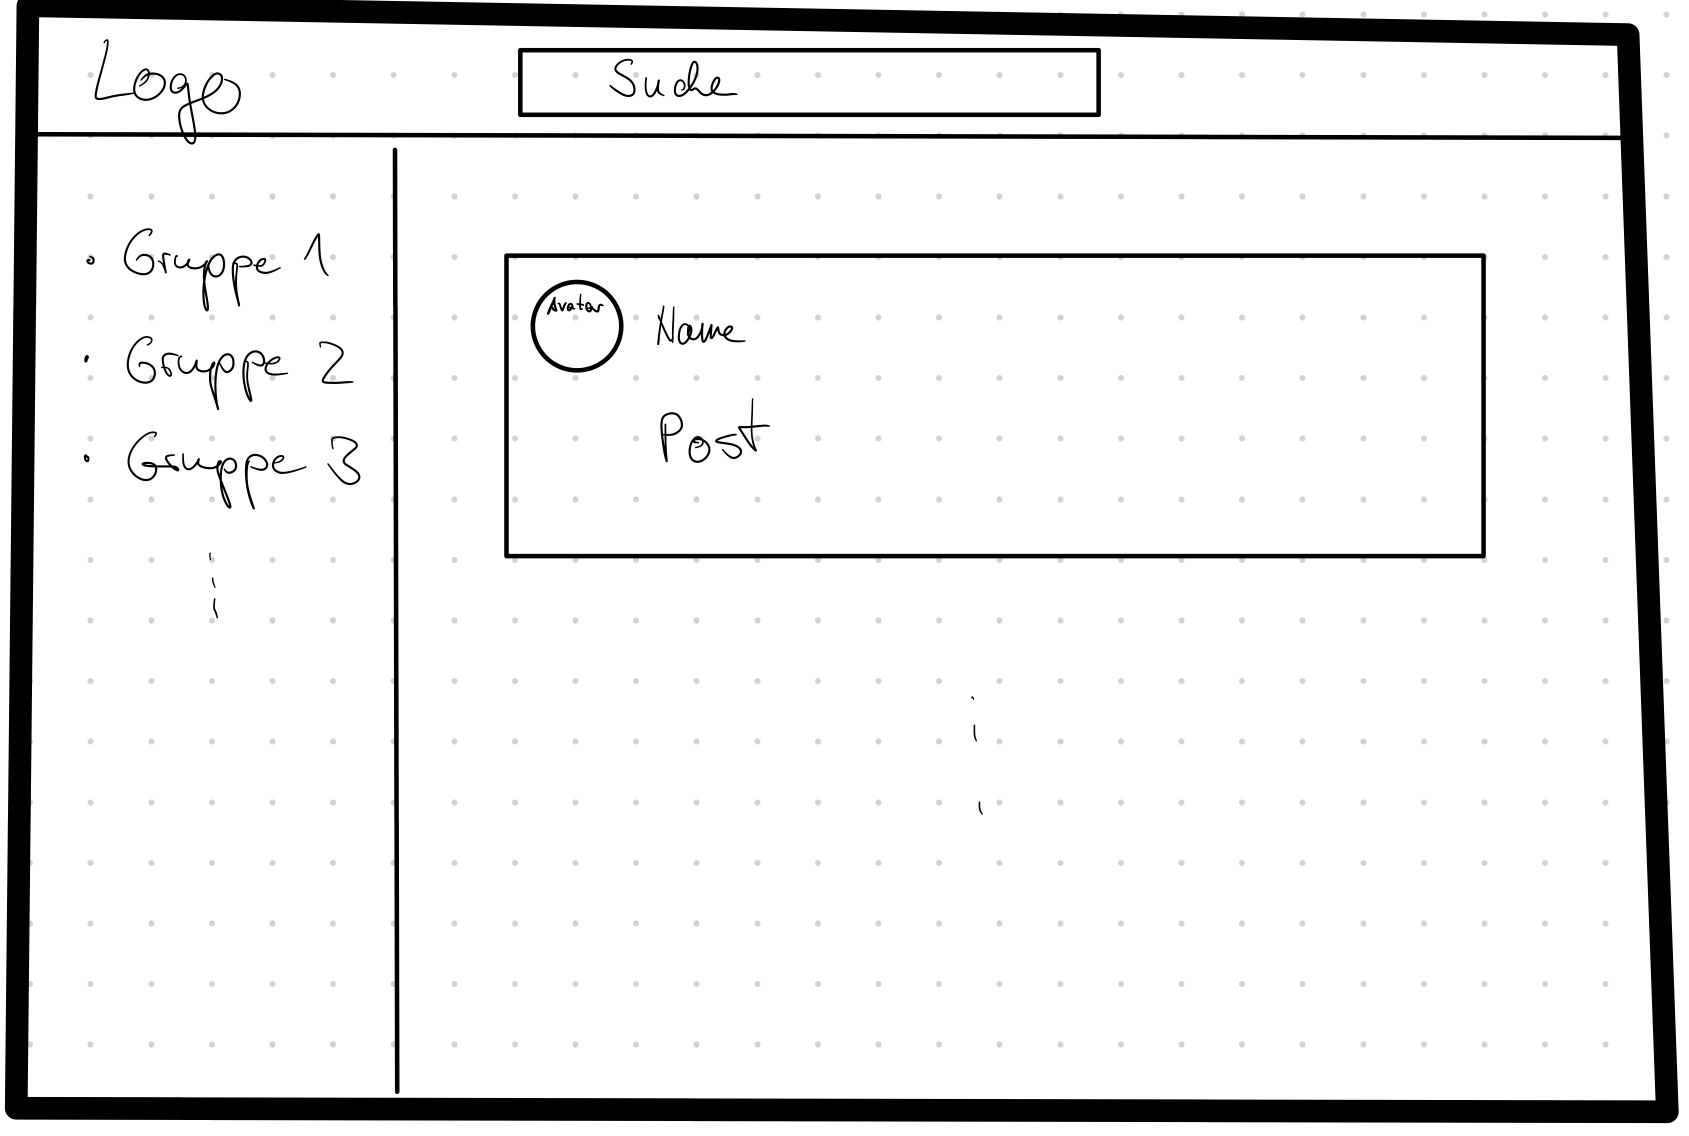
\includegraphics[scale = 0.2]{skizze.jpeg}
			\end{center}
		\end{itemize}
	\end{enumerate}
	
\end{document}